%%%%
% Consiglio la visione dei seguenti tutorial:
% - https://www.youtube.com/watch?v=ihxSUsJB_14
% - https://www.youtube.com/watch?v=XTFWaV55uDo
%%%%
\documentclass[12pt,a4paper,openright,twoside]{book}
\usepackage[utf8]{inputenc}

\newcommand{\thesislang}{italian} % decommentare in caso di tesi in italiano
%\newcommand{\thesislang}{english} % commentare in caso di tesi in italiano
\usepackage{thesis-style}

\begin{document}
	
\frontmatter

% ! TeX root = thesis-main.tex
\title{Title}
\author{Candidate Name Here}
\date{\today}

\begin{titlepage}
	\begin{center}
		% \vspace*{0.2cm}
		
		\large
		\textbf{ALMA MATER STUDIORUM -- UNIVERSITÀ DI BOLOGNA \\ CAMPUS DI CESENA}
		\\
		\noindent\hrulefill
		\vspace{0.4cm}
		
		\Large
		Scuola di Ingegneria e Architettura \\
		Corso di Laurea Magistrale in Ingegneria e Scienze Informatiche
		
		\Huge
		\vspace{4cm}
		\textbf{Assignment \#01}
		
		\large
		\vspace{1cm}
		Elaborato in 
		\\
		\textsc{Programmazione concorrente e distribuita}
		
		\vspace{5.5cm}
		\begin{minipage}[t]{0.64\textwidth}
			\begin{flushleft}
			\end{flushleft}
		\end{minipage}
		\begin{minipage}[t]{0.34\textwidth}
			\begin{flushright}
				\textit{Studenti} 
				\\ 
				\textbf{Eddie Barzi}
				\\ 
				\textbf{Filippo Vissani}
			\end{flushright}
		\end{minipage}\\
		
		\vfill
		\noindent\hrulefill
		\vspace{0.3cm}
		\Large

		Anno Accademico 2021-2022
	\end{center}
\end{titlepage}
\restoregeometry


%----------------------------------------------------------------------------------------
\tableofcontents   
%\listoffigures     % (optional) comment if empty
%\lstlistoflistings % (optional) comment if empty
%----------------------------------------------------------------------------------------

\mainmatter

%----------------------------------------------------------------------------------------
\chapter{\introductionname}
\label{chap:introduction}
%----------------------------------------------------------------------------------------
\section{Descrizione}
Viene fornito il codice di un programma che simula il movimento di $N$ corpi su un piano bidimensionale,
soggetti a due tipi di forze:
\begin{itemize}
	\item una forza repulsiva, per cui ogni corpo $b_{i}$ esercita su ogni altro corpo $b_{j}$ una forza in modulo pari a:
	\begin{center}
		$ F_{ij} = \frac{k_{rep} \times m_{i}}{d^2_{ij}} $
	\end{center}
	Dove $m_{i}$ è la massa del corpo $b_{i}$, $k_{rep}$ è una costante data, $d_{ij}$ è la distanza fra i due corpi.
	La direzione della forza è data dal versore $(b_{i} - b_{j})$, ovvero respingente per il corpo $b_{j}$.
	\item Una forza di attrito, per cui su ogni corpo $b_{i}$ che si muove a una velocità $v_{i}$ è esercitata una forza:
	\begin{center}
		$ FR_{i} = - k_{fri} \times v_{i} $
	\end{center}
	Che si oppone al moto, quindi in direzione opposta alla sua velocità, dove $k_{fri}$ è una costante data.
\end{itemize}
Il programma è sequenziale, non strutturato. 
L'algoritmo \ref{lst:lst1} definisce il comportamento del simulatore in pseudo codice.
\newpage
\begin{lstlisting}[label=lst:lst1,caption=Pseudocodice del programma sequenziale]
/* virtual time */
vt = 0;
/* time increment at each iteration */     
dt  = 0.01;

loop:
	for each body b[i]:
		compute total force exerted by other bodies b[j] and friction;
		compute the instant acceleration, given the total force and mass;
		update body velocity, given the acceleration and the virtual time elapsed dt;
	update bodies positions, given the velocity and virtual time elapsed dt;
	check boundary collisions;
	vt = vt + dt;   
	display current stage;

\end{lstlisting}

Alcuni aspetti rilevanti in merito al comportamento del programma e alla natura del problema:
\begin{itemize}
	\item Il calcolo delle forze al tempo $t$ avviene considerando coerentemente le posizioni dei corpi al tempo $t$. 
	\item L'aggiornamento delle posizioni può avvenire solo dopo che tutte le forze sono state calcolate (e le velocità aggiornate).
	\item Il controllo della collisione con i confini del mondo per un corpo $b_{i}$ può comportare il cambiamento della velocità e posizione del corpo.
	\item Nel programma, la visualizzazione dello stato corrente della simulazione o frame (via GUI) avviene in modo sincrono, per cui la successiva iterazione avviene solo dopo aver visualizzato lo stato della precedente.
\end{itemize}

\section{Obiettivi}
\subsection{Realizzazione di una Versione Concorrente della Simulazione}
Realizzare una versione concorrente della simulazione senza GUI, considerando un insieme iniziale $N$ di corpi
- e calcolando l'evoluzione temporale per un certo numero di passi $Nsteps$ -
con $Nsteps$ fissato come parametro. Posizione e velocità iniziali possono essere definite in modo casuale.
L'obiettivo è:
\begin{itemize}
	\item Massimizzare le performance, sfruttando tutte le capacità di calcolo del generico
	sistema di elaborazione su cui è mandato in esecuzione il programma.
	\item Organizzare il programma in modo modulare, estendibile.
\end{itemize}

Analizzare le performance del programma considerando valori di $N$ pari a 100, 1000, 5000, con $Nsteps$ pari a 1000, 10000, 50000,
calcolando lo speedup, e valutando il suo comportamento usando sia il numero ottimale teorico di thread,
sia considerando prove diverse con un numero variabile di threads per verificarne la scalabilità.
Verificare la correttezza del programma usando Java Path Finder, considerando la parte più significativa in merito, opportunamente semplificata.

\subsection{Inclusione di un'Interfaccia Grafica}
Estendere la simulazione includendo una GUI con pulsanti start/stop per lanciare/fermare la simulazione e visualizzare l'andamento,
includendo informazioni circa il tempo virtuale.
La GUI si presuppone visualizzi stati consistenti della simulazione (ma non necessariamente tutti gli stati).
%----------------------------------------------------------------------------------------
\chapter{Analisi del Problema}
\label{chap:Analisi del Problema}
%----------------------------------------------------------------------------------------
Portando il programma da sequenziale a parallelo devono essere considerati i seguenti aspetti:
\begin{itemize}
	\item Più flussi di esecuzione accedono in modo concorrente alla stessa lista di corpi.
	Quindi è necessario che i flussi siano sincronizzati (evitando deadlock, race contition, ecc...).
	\item La sincronizzazione deve avvenire in modo efficiente; bisogna sfruttare al massimo il tempo per
	la computazione evitando attese non necessarie.
	\item A ogni iterazione, dati due flussi di esecuzione $f_{i}$ e $f_{j}$, i quali eseguono computazioni su due corpi $c_{k}$ e $c_{w}$ rispettivamente (con $i \neq j$ e $k \neq w$),
	$f_{i}$ non deve aggiornare la posizione di $c_{k}$ prima che $f_{j}$ abbia terminato di calcolare la forza esercitata su $c_{w}$.
	\item La rappresentazione della simulazione deve rimanere
	consistente, i flussi devono essere sempre sincronizzati sulla
	stessa iterazione.
	\item È fondamentale che il numero di flussi di esecuzione venga scelto sulla base dei processori disponibili sulla macchina, ovvero
	rispettando la formula $N_{cpu} + 1$, per minimizzare il tempo di esecuzione.
	\item È buona pratica separare i componenti che riguardano la concorrenza dagli aspetti di logica e di grafica,
	così da rendere il sistema modulare ed estendibile.
	\item Gli eventi relativi alla pressione dei pulsanti
	devono essere gestiti atomicamente, dato che si occupano di
	avviare e fermare i flussi di esecuzione.
	\item Al termine della simulazione, sia nel caso in cui sia stato raggiunto
	il numero massimo di iterazioni, che nel caso in cui sia stato premuto il
	pulsante Stop, tutti i flussi di esecuzione devono terminare correttamente.
\end{itemize}

%----------------------------------------------------------------------------------------
\chapter{Descrizione dell'Architettura Proposta}
\label{chap:Descrizione dell'Architettura Proposta}
%----------------------------------------------------------------------------------------

In fase di progettazione, per separare al meglio gli aspetti di logica e grafica da quelli di concorrenza, si è scelto di
impiegare il pattern architetturale \textit{Model View Controller} (Figura \ref{fig:mvc}).
Nel \textit{Model} viene gestito l'aggiornamento della posizione dei corpi a ogni iterazione. In particolare viene fornita 
un'interfaccia di programmazione con i seguenti metodi (vengono riportati solo i più significativi):
\begin{itemize}
	\item \texttt{checkAndSolveBoundaryCollisionOnBodiesRange(range)}: 
	utilizzato per risolvere le collisioni di un intervallo di corpi con i bordi della simulazione.
	\item \texttt{updatePositionOnBodiesRange(range)}:
	utilizzato per aggiornare la posizione di un intervallo di corpi.
	\item \texttt{computeAccelerationOnBodiesRange(range)}:
	utilizzato per calcolare l'accelerazione di un intervallo di corpi.
	\item \texttt{updateSpeedOnBodiesRange(range, acceleration)}:
	utilizzato per aggiornare la velocità di un intervallo di corpi.
\end{itemize}
Nei metodi appena descritti viene specificato sempre l'intervallo di corpi per permettere ai worker di agire su porzioni 
differenti della lista senza generare race condition.

Gli aspetti di concorrenza vengono gestiti completamente nel \textit{Controller},
descritto più dettagliatamente in Figura \ref{fig:SimulatioManager}.
La classe \texttt{SimulationManager}, che implementa l'interfaccia \texttt{Runnable},
si occupa di generare i \texttt{Worker}, i quali a ogni iterazione
calcolano la nuova posizione dei corpi.
I \texttt{Worker} sono sincronizzati tra loro e con il \texttt{SimulationManager}
grazie a tre monitor di tipo barriera.
Nel Listato \ref{lst:lst3} viene riportata l'implementazione del metodo \texttt{await()} della classe \texttt{BarrierImpl}.
In questa implementazione l'ultimo thread che colpisce la barriera:
\begin{itemize}
	\item Risveglia tutti i thread che stanno attendendo.
	\item Imposta un flag che viene utilizzato per azzerare il campo
	che memorizza il numero di thread che hanno colpito la barriera.
	Questo perché le barriere vengono riutilizzate a ogni iterazione.
\end{itemize}

I worker e il simulation manager utilizzano un oggetto condiviso di tipo \texttt{AtomicBoolean}, 
il quale permette di terminare correttamente i flussi di esecuzione alla fine della simulazione.

Inoltre il \textit{Controller} si occupa di aggiornare la \textit{View} ad ogni iterazione.

\begin{figure}
	\centering
	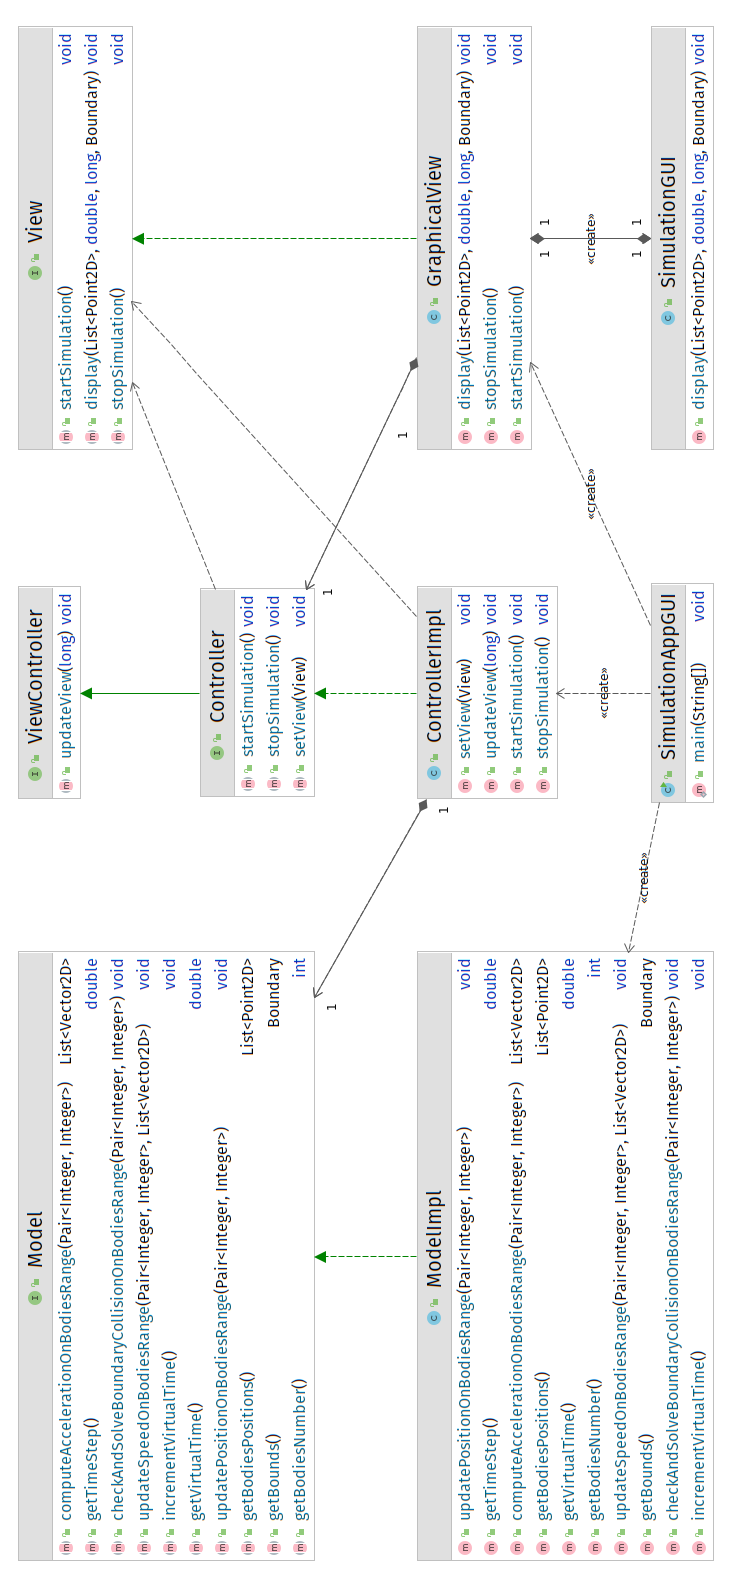
\includegraphics[width=0.6\linewidth]{figures/MVC-class-diagram.png}
	\caption{Model View Controller: diagramma delle classi.}
	\label{fig:mvc}
\end{figure}

\begin{figure}
	\centering
	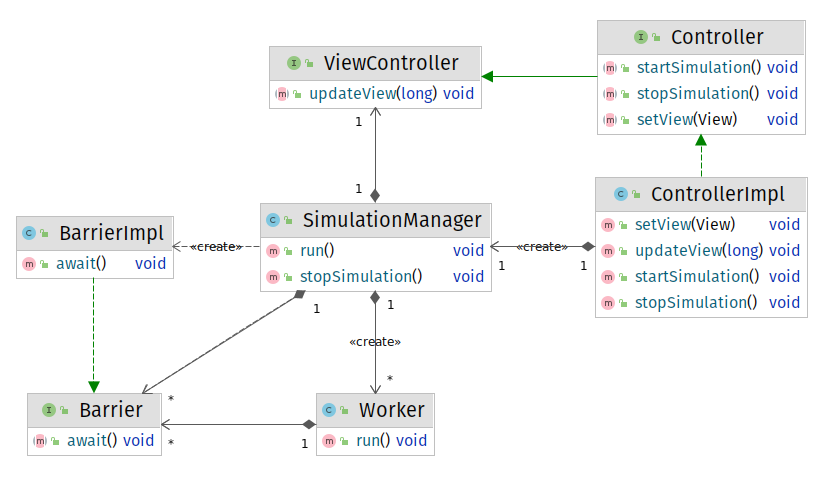
\includegraphics[width=\linewidth]{figures/simulation-manager.png}
	\caption{Controller: diagramma delle classi.}
	\label{fig:SimulatioManager}
\end{figure}

\begin{lstlisting}[float,
					language=Java,
					label=lst:lst3,caption=Implementazione della barrier]
public synchronized void hitAndWaitAll() throws InterruptedException {
	this.actualWorkers = this.actualWorkers + 1;
	if (this.actualWorkers == this.workersNumber) {
		this.exit = true;
		notifyAll();
	} else {
		while (this.actualWorkers < this.workersNumber && !this.exit) {
			wait();
		}
	}
	this.actualWorkers = this.actualWorkers - 1;
	if (this.actualWorkers == 0) this.exit = false;
}
\end{lstlisting}

La \textit{View} (Figura \ref{fig:gui}) oltre a rappresentare lo stato corrente della simulazione, 
riporta il tempo virtuale e l'iterazione attuali.
L'interfaccia grafica dispone anche di due pulsanti, utilizzati per avviare e fermare la simulazione.

\begin{figure}
	\centering
	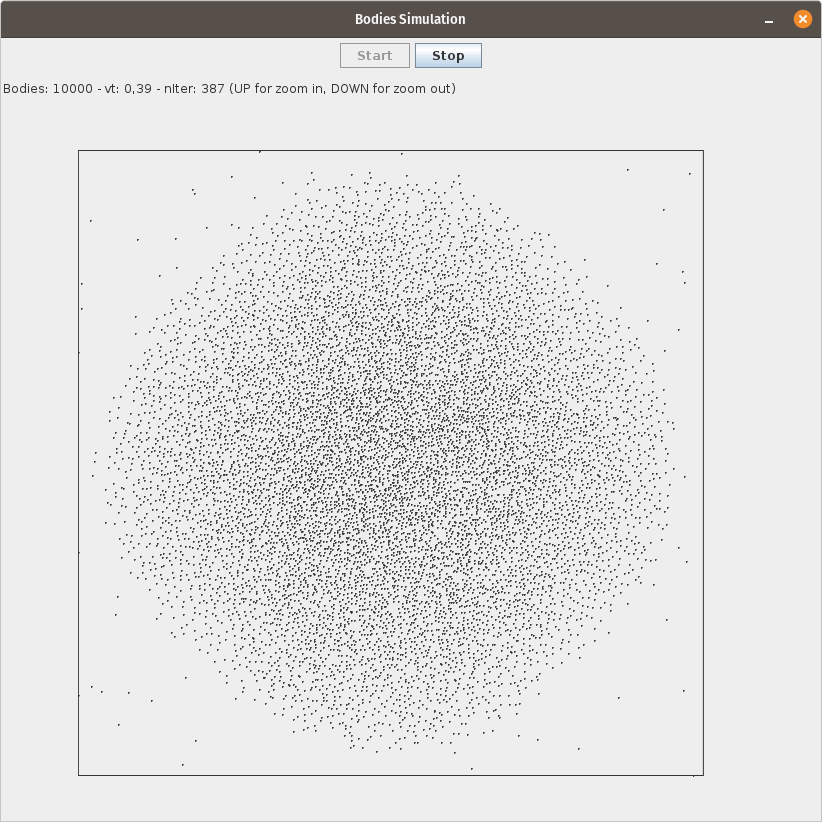
\includegraphics[width=\linewidth]{figures/simulation.png}
	\caption{Interfaccia grafica}
	\label{fig:gui}
\end{figure}


%----------------------------------------------------------------------------------------
\chapter{Descrizione del Comportamento del Sistema} % possible chapter for Projects
\label{chap:Descrizione del Comportamento del Sistema}
%----------------------------------------------------------------------------------------
Nei listati \ref{lst:worker} e \ref{lst:simulation_manager} vengono riportati i comportamenti del worker e del simulation manager rispettivamente.

In Figura \ref{fig:petri-net} viene riportato il comportamento generale del simulation manager e di due worker (A e B) utilizzando 
le reti di Petri.

Vengono utilizzate tre barriere condivise tra il simulation manager e i worker:
\begin{enumerate}
	\item Inizialmente il simulation manager attende che i worker
	abbiano terminato di aggiornare le posizioni dei corpi
	e verificato le collisioni (istruzioni: R0 e R1).
	\item A ogni iterazione i worker prima aggiornano la velocità dei corpi,
	poi incontrano la prima barriera (istruzioni:P,Q 1).
	\item Dopo aver passato la prima barriera i worker aggiornano la posizione dei corpi,
	eseguono il controllo delle collisioni e incontrano la seconda barriera (istruzioni:P,Q 4).
	\item A questo punto i worker attendono nella terza barriera (istruzioni:P,Q 5) mentre il simulation
	manager aggiorna l'interfaccia grafica.
	\item Dopo l'aggiornamento dell'interfaccia grafica il simulation manager incontra
	la terza barriera (istruzione: R3) e inizia una nuova iterazione.

\newpage

\end{enumerate}
\begin{lstlisting}[label=lst:worker,caption=Pseudocodice del worker]
		while(!stop):
(P,Q)0:		update bodies speed
(P,Q)1:		barrier0.await()
(P,Q)2:		update bodies position
(P,Q)3:		check collisions
(P,Q)4:		barrier1.await()
(P,Q)5:		barrier2.await()
\end{lstlisting}

\begin{lstlisting}[label=lst:simulation_manager,caption=Pseudocodice del simulation manager]
		while(!stop):
R0:			barrier0.await()
R1:			barrier1.await()
R2:			update the view
R3:			barrier2.await()
\end{lstlisting}

\begin{figure}
	\centering
	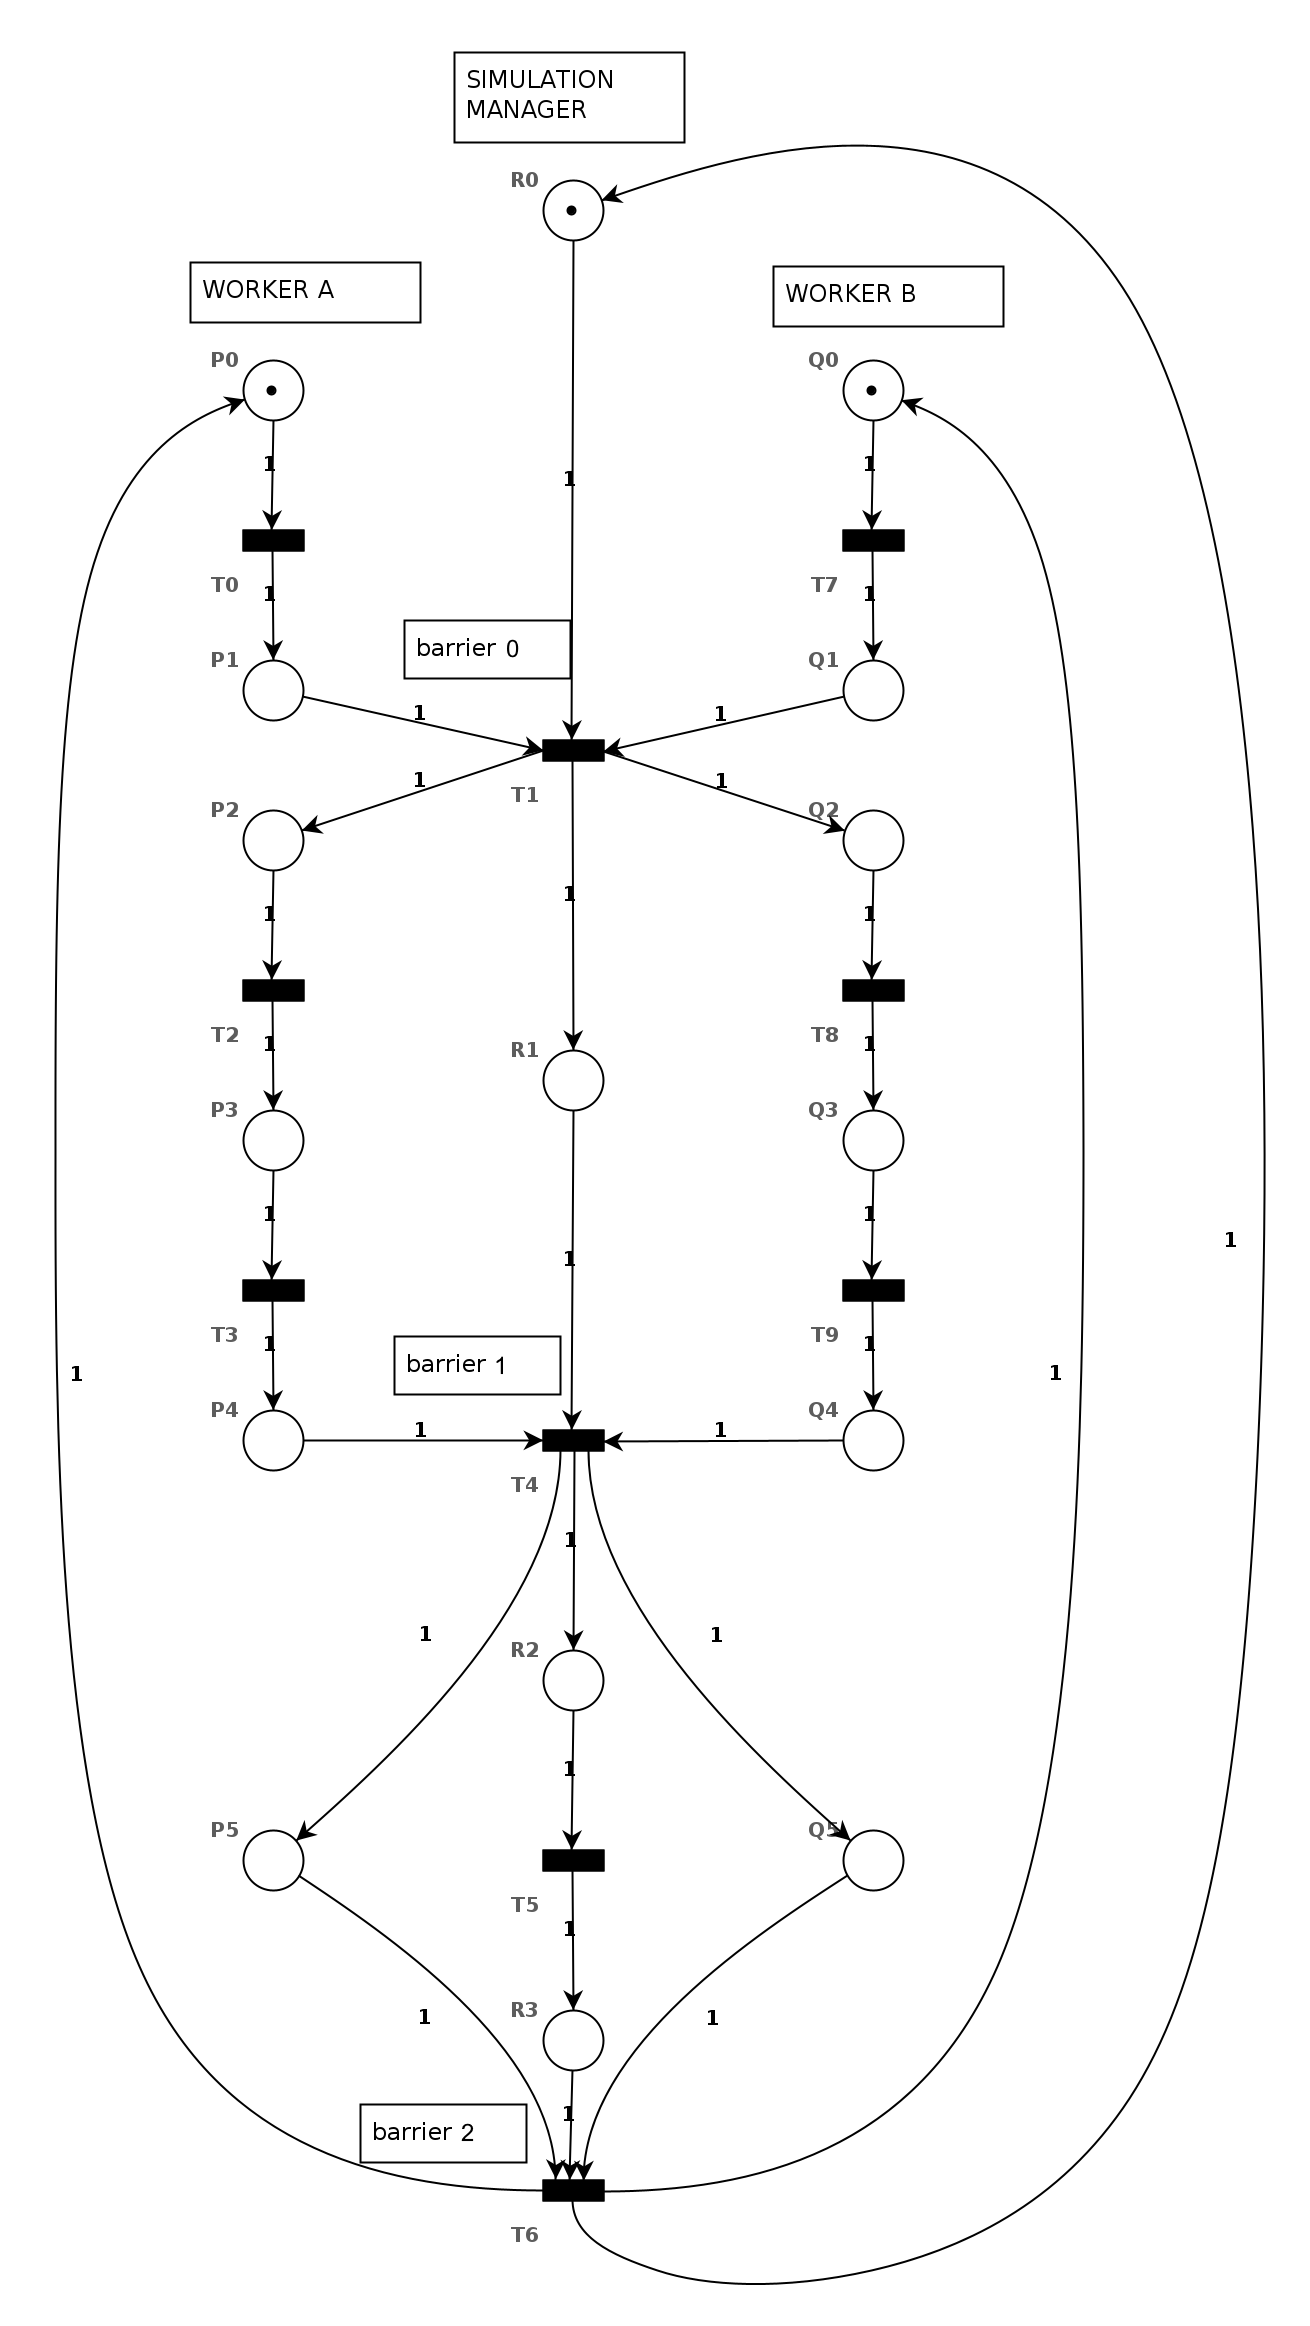
\includegraphics[width=0.7\linewidth]{figures/petri-net.png}
	\caption{Rete di Petri.}
	\label{fig:petri-net}
\end{figure}

%----------------------------------------------------------------------------------------
\chapter{Verifica delle Prestazioni} % possible chapter for Projects
\label{chap:Verifica delle Prestazioni}
%----------------------------------------------------------------------------------------

I test sono stati effettuati su una macchina con le seguenti caratteristiche:
\begin{itemize}
	\item Sistema operativo: Fedora 35 (GNU/Linux)
	\item Versione kernel Linux: 5.16.18
	\item Memoria: 16GB, 3200Mhz
	\item CPU: AMD Ryzen 7 5700U
\end{itemize}
Descrizione dettagliata del processore:
\begin{itemize}
	\item Core: 8
	\item Thread: 16
	\item Clock base: 1.8GHz
	\item Clock max: 4.3GHz
	\item Cache L2: 4MB
	\item Cache L3: 8MB
\end{itemize}

Osservando i dati riportati nella Tabella \ref{tab:table1}
si possono trarre le seguenti conclusioni:
\begin{itemize}
	\item Per un numero di corpi sufficientemente piccolo (in questo caso 100),
	il programma sequenziale impiega meno tempo di quello concorrente.
	\item $N_{cpu}+1$ risulta essere il numero ottimale di thread da utilizzare
	solo con un numero elevato di corpi. In ogni caso prestazioni simili possono essere raggiunte anche con meno thread (9).
	Le simulazioni con numero di corpi e iterazioni elevati, la differenza dei tempi di esecuzione tra 9 e 17 thread è minima.
	\item Impiegare un numero elevato di thread non porta a un incremento significativo delle prestazioni, al contrario, genera overhead.
\end{itemize}

In Figura \ref{fig:speedup} viene presentato un grafico che riporta l'andamento dello speedup in funzione del numero di corpi e di thread.

Aumentando notevolmente il numero di corpi (50000), anche con un numero basso di iterazioni,
la differenza dei tempi di esecuzione diventa rilevante.
I risultati dei test riportati in Tabella \ref{tab:table2} dimostrano effettivamente che
il numero ottimale di thread da utilizzare è $N_{cpu} + 1$, infatti c'è una differenza notevole tra le simulazioni con 9 e con 17 thread. 
In questo caso, la simulazione con un numero di thread elevato (99) risulta più veloce di quella con il numero ottimale di thread, anche se di poco.

\begin{table}[h!]
	\centering
	\begin{tabular}{ |c|c|c|c|c|c| } 
		\hline
		Numero test & Corpi & Iterazioni & Thread & Tempo esecuzione (ms) & Speedup \\
		\hline
		0 & 100 & 1000 & 1 & 157 & 1.0 \\ 
		\hline
		1 & 100 & 1000 & 9 & 201 & 0.78 \\ 
		\hline
		2 & 100 & 1000 & 17 & 600 & 0.26 \\ 
		\hline
		3 & 100 & 1000 & 99 & 3567 & 0.04 \\ 
		\hline
		4 & 100 & 10000 & 1 & 1171 & 1.0 \\ 
		\hline
		5 & 100 & 10000 & 9 & 3618 & 0.32 \\ 
		\hline
		6 & 100 & 10000 & 17 & 6582 & 0.18 \\ 
		\hline
		7 & 100 & 10000 & 99 & 33952 & 0.03 \\ 
		\hline
		8 & 100 & 50000 & 1 & 5283 & 1.0 \\ 
		\hline
		9 & 100 & 50000 & 9 & 13822 & 0.38 \\ 
		\hline
		10 & 100 & 50000 & 17 & 32673 & 0.16 \\ 
		\hline
		11 & 100 & 50000 & 99 & 167340 & 0.03 \\ 
		\hline
		12 & 1000 & 1000 & 1 & 8296 & 1.0 \\ 
		\hline
		13 & 1000 & 1000 & 9 & 4324 & 1.92 \\ 
		\hline
		14 & 1000 & 1000 & 17 & 4773 & 1.74 \\ 
		\hline
		15 & 1000 & 1000 & 99 & 5174 & 1.6 \\ 
		\hline
		16 & 1000 & 10000 & 1 & 82545 & 1.0 \\ 
		\hline
		17 & 1000 & 10000 & 9 & 42564 & 1.94 \\ 
		\hline
		18 & 1000 & 10000 & 17 & 47085 & 1.75 \\ 
		\hline
		19 & 1000 & 10000 & 99 & 52254 & 1.58 \\ 
		\hline
		20 & 1000 & 50000 & 1 & 413015 & 1.0 \\ 
		\hline
		21 & 1000 & 50000 & 9 & 218415 & 1.89 \\ 
		\hline
		22 & 1000 & 50000 & 17 & 244789 & 1.69 \\ 
		\hline
		23 & 1000 & 50000 & 99 & 270243 & 1.53 \\ 
		\hline
		24 & 5000 & 1000 & 1 & 182638 & 1.0 \\ 
		\hline
		25 & 5000 & 1000 & 9 & 104925 & 1.74 \\ 
		\hline
		26 & 5000 & 1000 & 17 & 103332 & 1.77 \\ 
		\hline
		27 & 5000 & 1000 & 99 & 105752 & 1.73 \\ 
		\hline
		28 & 5000 & 10000 & 1 & 1925941 & 1.0 \\ 
		\hline
		29 & 5000 & 10000 & 9 & 1033744 & 1.86 \\ 
		\hline
		30 & 5000 & 10000 & 17 & 1028930 & 1.87 \\ 
		\hline
		31 & 5000 & 10000 & 99 & 1067935 & 1.8 \\ 
		\hline
		32 & 5000 & 50000 & 1 & 10226313 & 1.0 \\ 
		\hline
		33 & 5000 & 50000 & 9 & 5163395 & 1.98 \\ 
		\hline
		34 & 5000 & 50000 & 17 & 5115270 & 2.0 \\ 
		\hline
		35 & 5000 & 50000 & 99 & 5311090 & 1.93 \\ 
		\hline
	\end{tabular}
	\caption{Risultati dei test}
	\label{tab:table1}
\end{table}

\begin{figure}
	\centering
	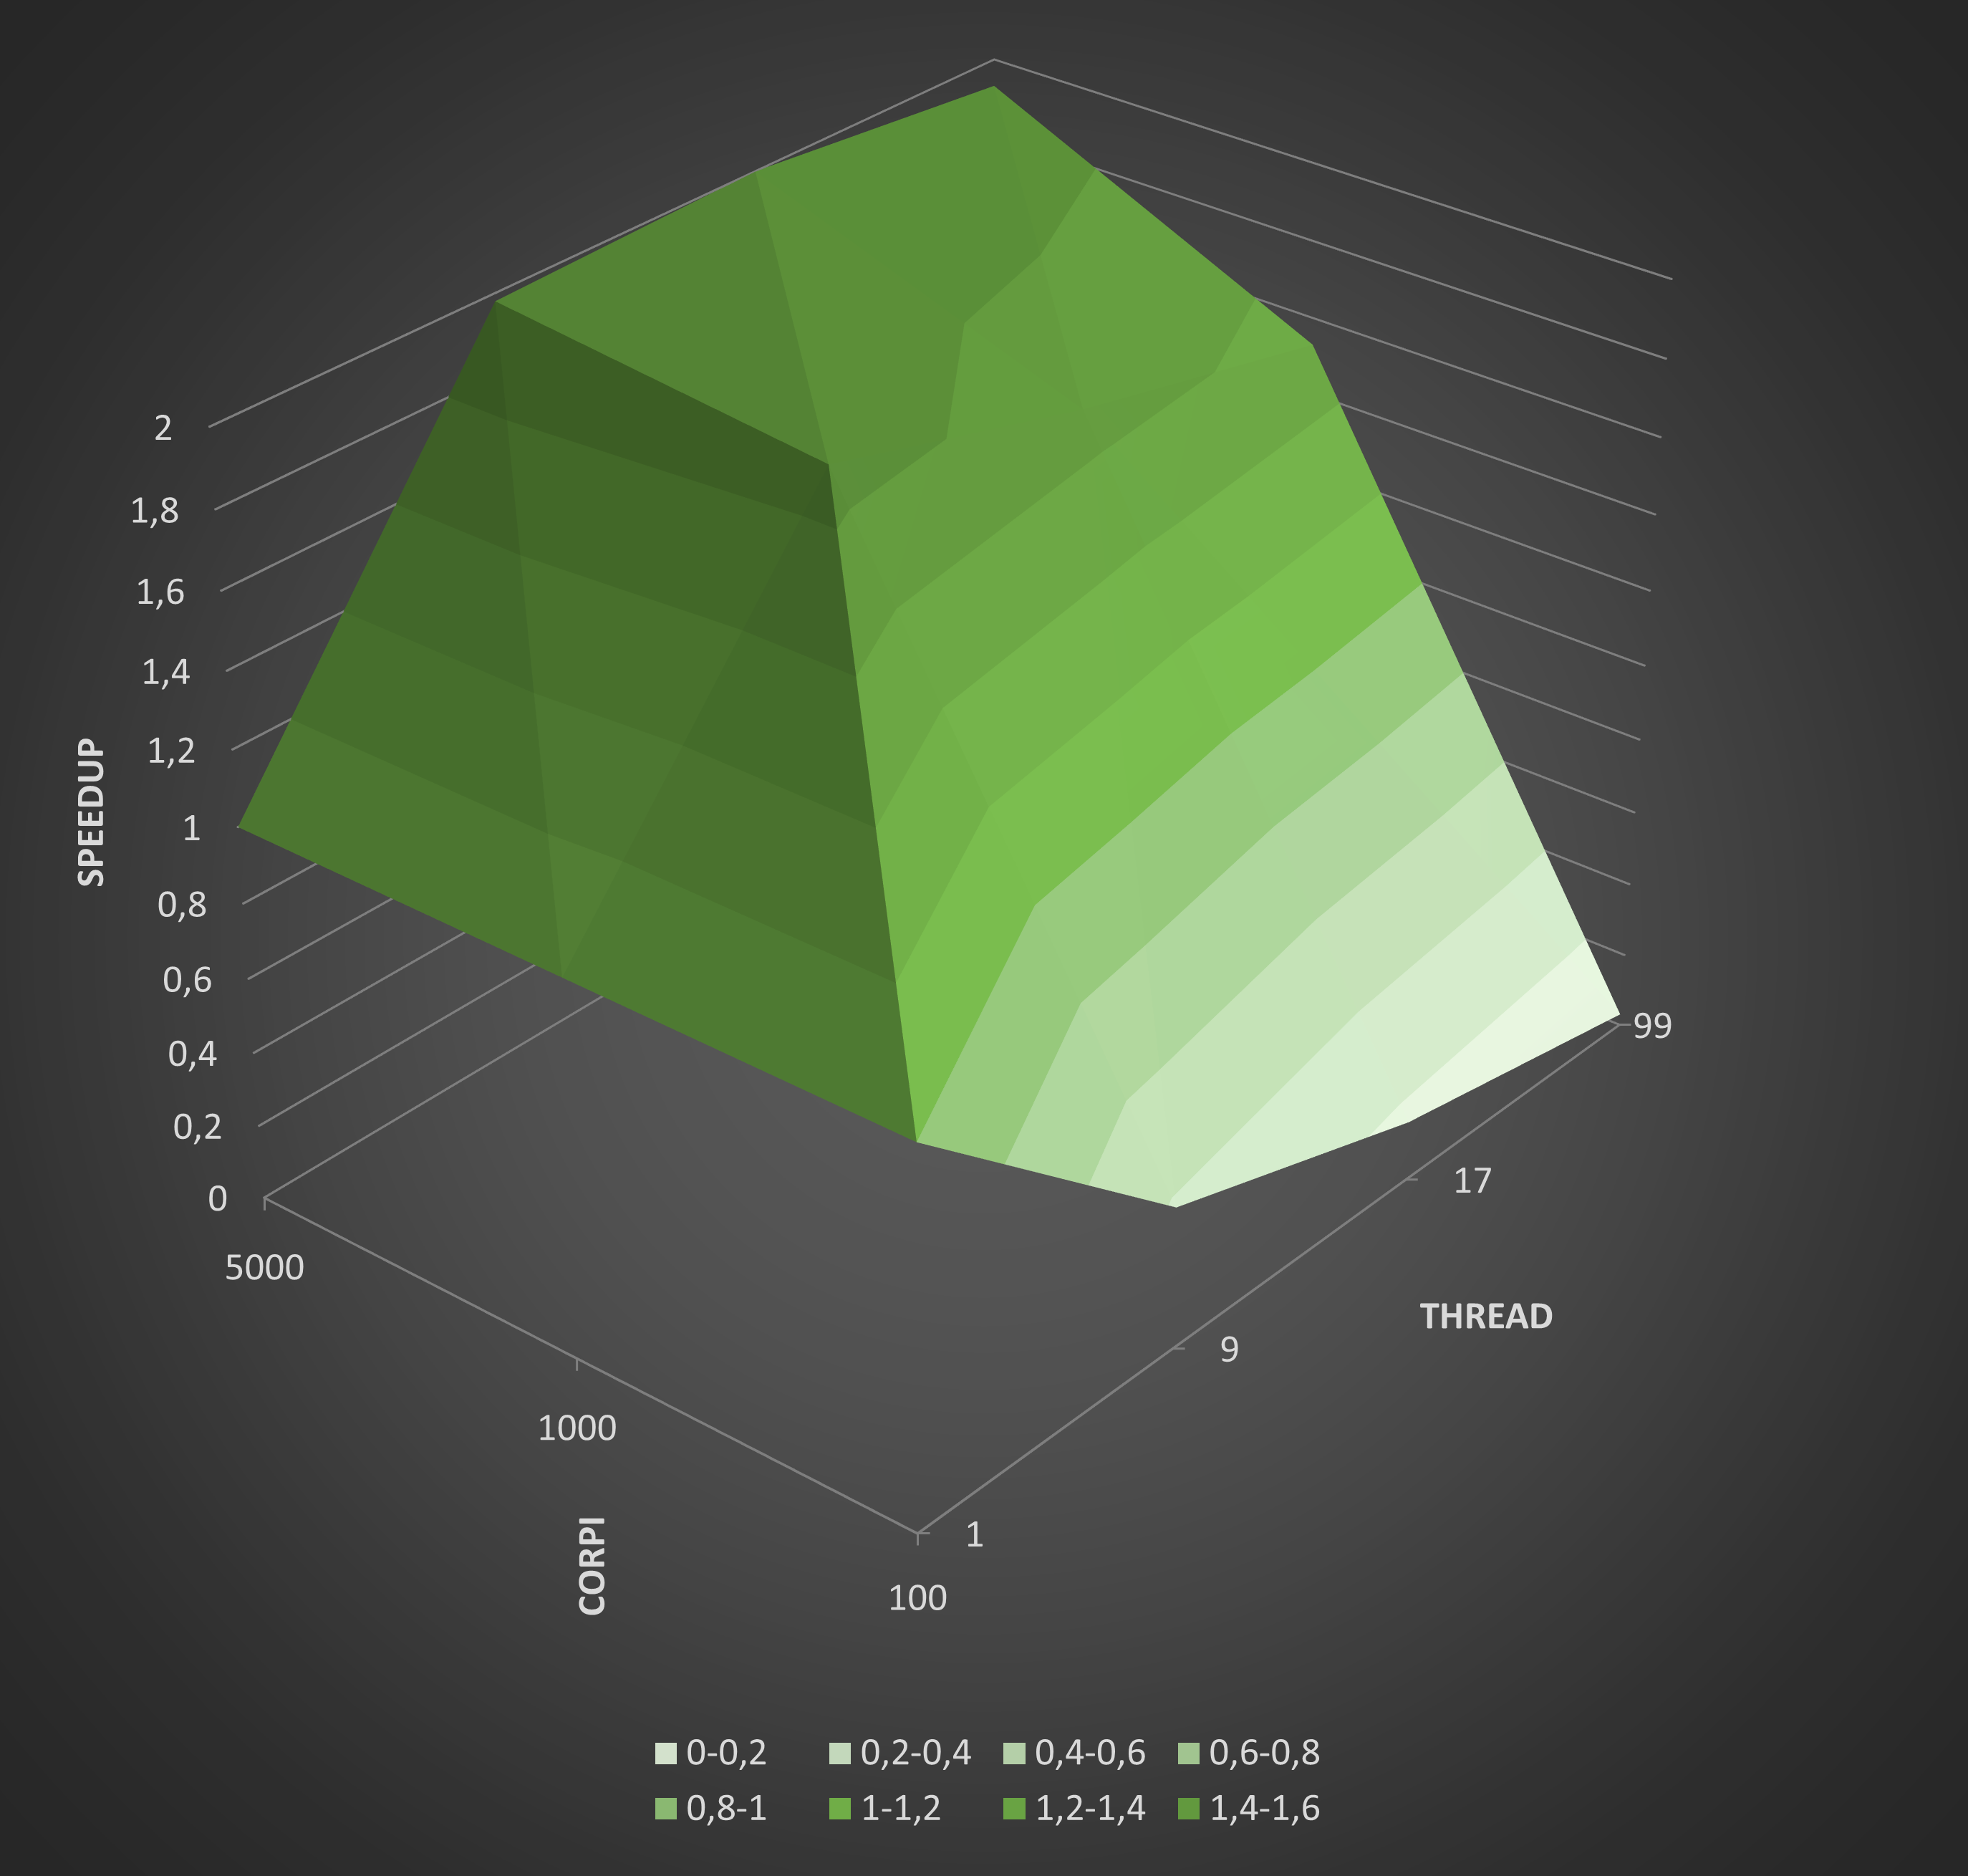
\includegraphics[width=0.9\linewidth]{figures/speedup-plot.png}
	\caption{Speedup in funzione del numero di thread e di corpi (con numero di iterazioni fissato a 50000).}
	\label{fig:speedup}
\end{figure}

\begin{table}[h!]
	\centering
	\begin{tabular}{ |c|c|c|c|c|c| } 
		\hline
			Numero test & Corpi & Iterazioni & Thread & Tempo esecuzione (ms) & Speedup \\
		\hline
		36 & 50000 & 100 & 1 & 7602654 & 1.0 \\ 
		\hline
		37 & 50000 & 100 & 9 & 1596103 & 4.76 \\ 
		\hline
		38 & 50000 & 100 & 17 & 1326848 & 5.73 \\ 
		\hline
		39 & 50000 & 100 & 99 & 1285153 & 5.92 \\ 
		\hline
	\end{tabular}
	\caption{Risultati dei test}
	\label{tab:table2}
\end{table}

%----------------------------------------------------------------------------------------
\chapter{Identificazione delle Proprietà di Correttezza} % possible chapter for Projects
\label{chap:Identificazione delle Proprietà di Correttezza}
%----------------------------------------------------------------------------------------
Per verificare la correttezza del programma è stato utilizzato Java Path Finder,
un tool che esegue il model checking del programma per trovare eventuali problemi relativi alla concorrenza,
quali deadlock e race condition.
L'analisi del programma con JPF ha prodotto il risultato desiderato (Figura \ref{fig:jpf-test}), nessun errore è stato rilevato.

\begin{lstlisting}[label=lst:jpf-file,caption=File JPF]
	target = pcd.assignment01.concurrent.simulation.SimulationApp

	classpath = build/classes/java/main
	
	listener = gov.nasa.jpf.listener.PreciseRaceDetector
	
	report.console.property_violation = error,trace
\end{lstlisting}


\begin{figure}
	\centering
	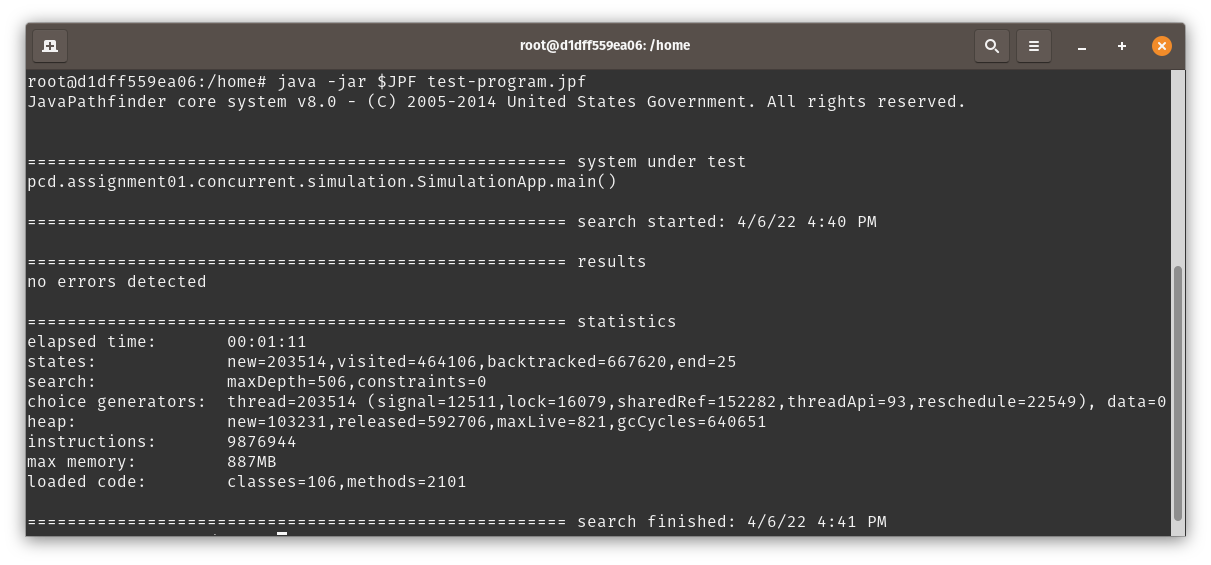
\includegraphics[width=\linewidth]{figures/jpf-test.png}
	\caption{Risultato dell'esecuzione di JPF sul sistema}
	\label{fig:jpf-test}
\end{figure}

\end{document}